% econ-slides Beamer alternate for Presentation 2 (progress report).
% Companion to slides/build_presentation2_deck.py (the python-pptx version);
% this is a second option, not a replacement. See structure-plan.md.
% Compile: python3 ~/.claude/skills/econ-slides/scripts/compile_deck.py talk.tex
\documentclass[11pt, aspectratio=169]{beamer}
\usepackage{econ-slides-house}
% Shared title metadata and result phrases for talk.tex and script.tex.
% Every magnitude below is sourced from progress_brief.tex (P2's results
% write-up); background/model phrasing is sourced from research_brief.tex.
% Numbers are never rounded further for the slide than they are in the brief.

\newcommand{\PaperTitle}{Network Position and Academic Performance\\[0.15em]
  {\normalsize Adding Network Centrality to Smirnov \& Thurner (2017)}}
\newcommand{\PaperShortTitle}{Network Position and Academic Performance}
\newcommand{\PaperAuthors}{Amy Bing \and Tingying Huang}
\newcommand{\AuthorShort}{Bing \& Huang}
\newcommand{\PresenterName}{Tingying Huang}
\newcommand{\CoauthorsSpoken}{Amy Bing}
\newcommand{\PaperAffiliations}{Monash University}
% Shared affiliation for both authors -- the simple default path (no
% per-author \AuthorAffil tabular needed since both are Monash).
\newcommand{\TitleAuthorBlock}{\PaperAuthors}
\newcommand{\TitleAffiliationBlock}{\PaperAffiliations}
\newcommand{\KeyQuestion}{Does network position predict grades?}
\newcommand{\KeyQuestionSubtitle}{On top of who a student's direct friends are}
\newcommand{\VenueDate}{ECC3841 Network Economics}
\newcommand{\VenueShort}{Presentation 2 --- Progress Report}
\newcommand{\TitleDisclaimer}{}

% ---- Result phrases: slide (written) and spoken (script) forms share the ----
% ---- same source-traced number, worded for the medium.                  ----

% Result 1 -- replication. Source: progress_brief.tex, "Result 1".
\newcommand{\ResultOneSlide}{Own past GPA strongly predicts next GPA ($\beta=0.955$); a friend's past GPA does not (\(p=0.557\))}
\newcommand{\ResultOneSpoken}{a student's own past GPA is a very strong predictor of their next GPA, but once you control for that, a friend's past GPA predicts nothing}

% Result 2 -- naive effect is popularity. Source: progress_brief.tex, "Result 2".
\newcommand{\ResultTwoSlide}{Katz-Bonacich alone: $+0.093$ ($p<0.001$). Add degree: $-0.028$ ($p=0.446$)}
\newcommand{\ResultTwoSpoken}{on its own, centrality looks like it matters, but the moment you add raw popularity to the same regression, that effect disappears}

% Result 3 -- pooled headline, read at face value. Source: progress_brief.tex, "Result 3".
\newcommand{\ResultThreeSlide}{$\beta=-0.0415$, SE\(=0.019\), \(p=0.033\), \(n=36{,}696\)}
\newcommand{\ResultThreeSpoken}{a small, negative, statistically significant effect, at the value of phi we fixed in advance}

% Result 4 -- corrected test. Source: progress_brief.tex, "Result 4".
\newcommand{\ResultFourSlide}{No \(\phi\) is significant ($p=0.36$ to $0.93$); the sign is not even consistent}
\newcommand{\ResultFourSpoken}{at every value of phi, not significant, and the sign flips back and forth}

% Headline / conclusion. Source: progress_brief.tex, boxed conclusion.
\newcommand{\ResultHeadlineSlide}{Net of popularity, friend GPA, and a student's own past performance, we find no evidence that network position independently predicts grades}
\newcommand{\ResultHeadlineSpoken}{once we properly control for popularity, friend GPA, and a student's own past performance, there is no evidence that network position predicts grades on its own}
\newcommand{\ResultSupportSlide}{Naive centrality looked positive, the pooled sweep looked negative, the corrected test looks like nothing}
\newcommand{\ResultSupportSpoken}{the naive test looked positive, the pooled test looked negative, and the one correctly specified test looks like nothing at all}
\newcommand{\ResultImplicationSlide}{Interventions built around widening students' network reach are not supported by this data once the obvious confounds are handled}
\newcommand{\ResultImplicationSpoken}{so policies that try to help students by widening their network reach are not supported by what we've found here}


% COLOR LEDGER: cTreatment = Katz-Bonacich centrality / network position (our
% added object vs. Smirnov & Thurner's baseline). cControl = own-past-GPA,
% the control at the center of the identification gap and its fix.
% Popularity/in-degree stays neutral black -- an inherited confound, not ours.
\colorlet{cTreatment}{cAccentA}
\colorlet{cControl}{cAccentC}

\title[\PaperShortTitle]{\PaperTitle}
\author[\AuthorShort]{\TitleAuthorBlock}
\institute{\TitleAffiliationBlock}
\date[\VenueShort]{\VenueDate \\ \VenueShort}

\begin{document}

\begin{frame}[plain]
  \titlepage
\end{frame}
\addtocounter{framenumber}{-1}

% ---- 1. Key question ----
\begin{frame}[t]{\KeyQuestion}
  \framesubtitle{\KeyQuestionSubtitle}
  \hypertarget{main:keyq}{}%
  \medskip
  \RunIn{Recap:} Smirnov \& Thurner (2017) show grades and friends' grades are
  linked mostly by \emph{selection}, not influence --- but they look at one
  number, a friend's average GPA. Calv\'o-Armengol, Patacchini \& Zenou (2009)
  show that \emph{position} (Katz--Bonacich centrality) predicts achievement
  --- but only in a single snapshot, so cause and effect are not separated.

  \medskip
  \RunIn{Our plan:} take the centrality prediction to Smirnov \& Thurner's
  panel data, and test it while holding friend-group GPA and a student's own
  past GPA fixed.

  \medskip
  \graycite{(Calv\'o-Armengol, Patacchini \& Zenou 2009; Smirnov \& Thurner 2017)}

  \PlaceNav{\hyperlink{app:lit}{\beamergotobutton{Related literature}}}
\end{frame}

% ---- 2. Recap: design and data ----
\begin{frame}[t]{Recap: design and data}
  \framesubtitle{The empirical strategy from Presentation 1}
  \hypertarget{main:datarecap}{}%
  \medskip
  \[
  \begin{aligned}
    \mathrm{GPA}_{i,t+1} = {}& \beta_0 + \beta_1\,\textcolor{cTreatment}{\mathrm{Katz}_{i,t}}
      + \beta_2\,\textcolor{cControl}{\mathrm{GPA}_{i,t}}
      + \beta_3\,\overline{\mathrm{GPA}}^{\,\text{friends}}_{i,t} \\[2pt]
      & {} + \beta_4\,\mathrm{InDeg}_{i,t} + \beta_5\,\mathrm{OutDeg}_{i,t}
      + \gamma_{\text{group}} + \varepsilon_{i,t}
  \end{aligned}
  \]
  \RunIn{Each control has a job:} friend GPA nets out friend-group
  composition; in- and out-degree net out raw popularity; \(\phi\) is swept
  from near 0 (popularity) to near its ceiling (long reach).

  \medskip
  \RunIn{The data:} 5 cohorts, 655--1,549 students each, directed ``like''
  ties every \(\sim\)3 months. \textbf{GPA repeats over time for the school
  group only} --- each university cohort has one static GPA value.
  \PlaceNav{\hyperlink{app:sample}{\beamergotobutton{Sample details}}}
\end{frame}

% ---- 3. What we did ----
\begin{frame}{What we did}
  \medskip
  \begin{enumerate}\setlength{\itemsep}{0.75em}
    \item \textbf{Replicate} --- confirm the data behaves the way Smirnov \&
      Thurner reported.
    \item \textbf{Naive test} --- centrality alone, no popularity control.
    \item \textbf{Planned test} --- add popularity, sweep \(\phi\), pool all
      5 groups.
    \item \textbf{Check \& fix} --- test the assumptions; found one had
      failed.
  \end{enumerate}
  \Takeaway{Here's what actually happened when we ran it.}
\end{frame}

% ---- 4. Result 1 ----
\begin{frame}{The replication holds}
  \framesubtitle{Own past GPA vs.\ a friend's past GPA, school group, \(n=2{,}088\)}
  \centering
  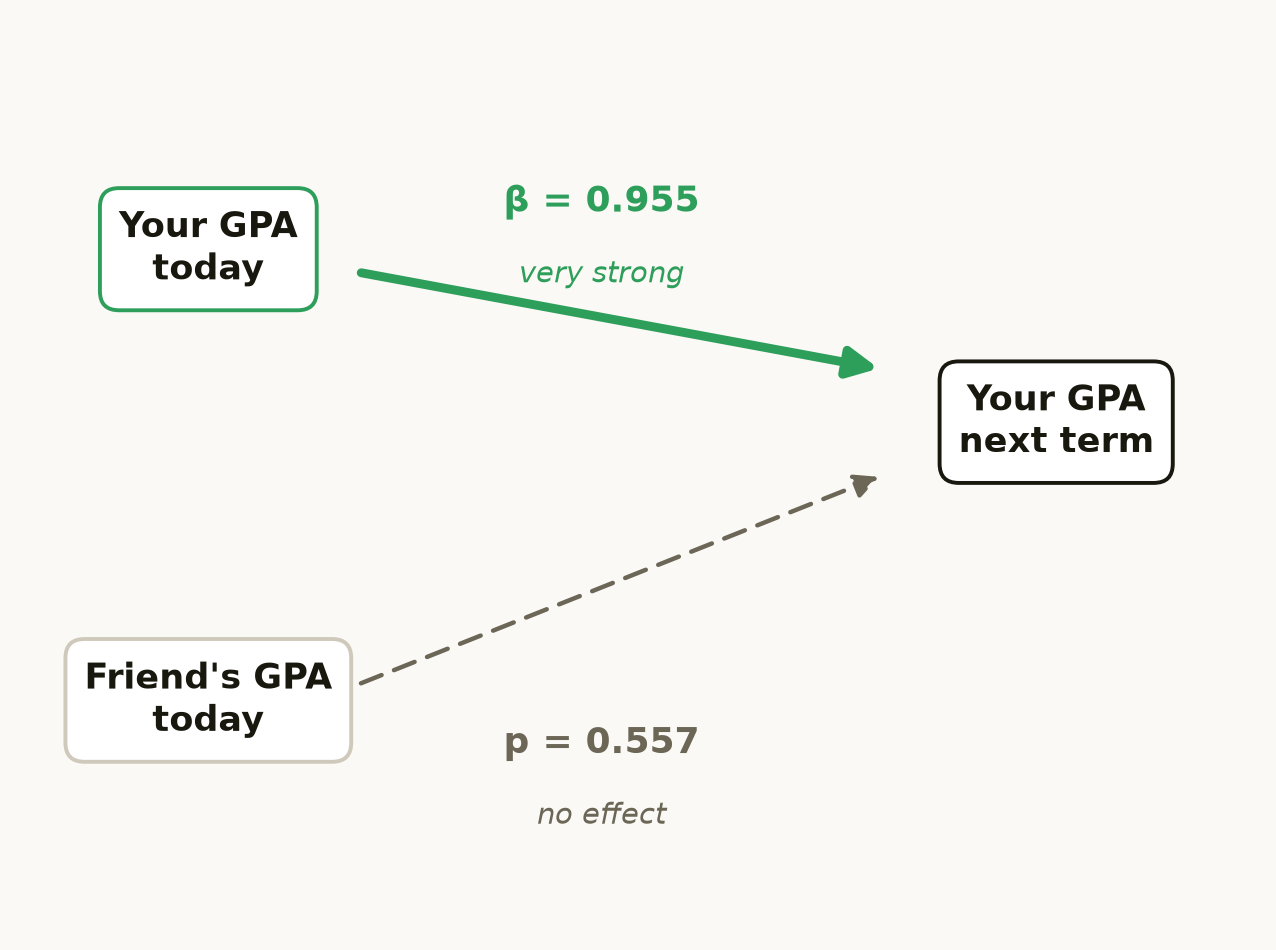
\includegraphics[height=0.6\textheight]{figures/fig_p2_result1_arrows.png}
  \Takeaway{New friendships are also more GPA-similar than dissolving ones
    (university \(p<0.001\); same direction in school, \(p=0.183\)). Both
    match Smirnov \& Thurner --- the foundation the rest of this talk builds
    on.}
\end{frame}

% ---- 5. Result 2 ----
\begin{frame}{The naive effect is popularity, relabelled}
  \framesubtitle{Katz-Bonacich alone vs.\ with a degree control, pooled, \(n=36{,}696\)}
  \centering
  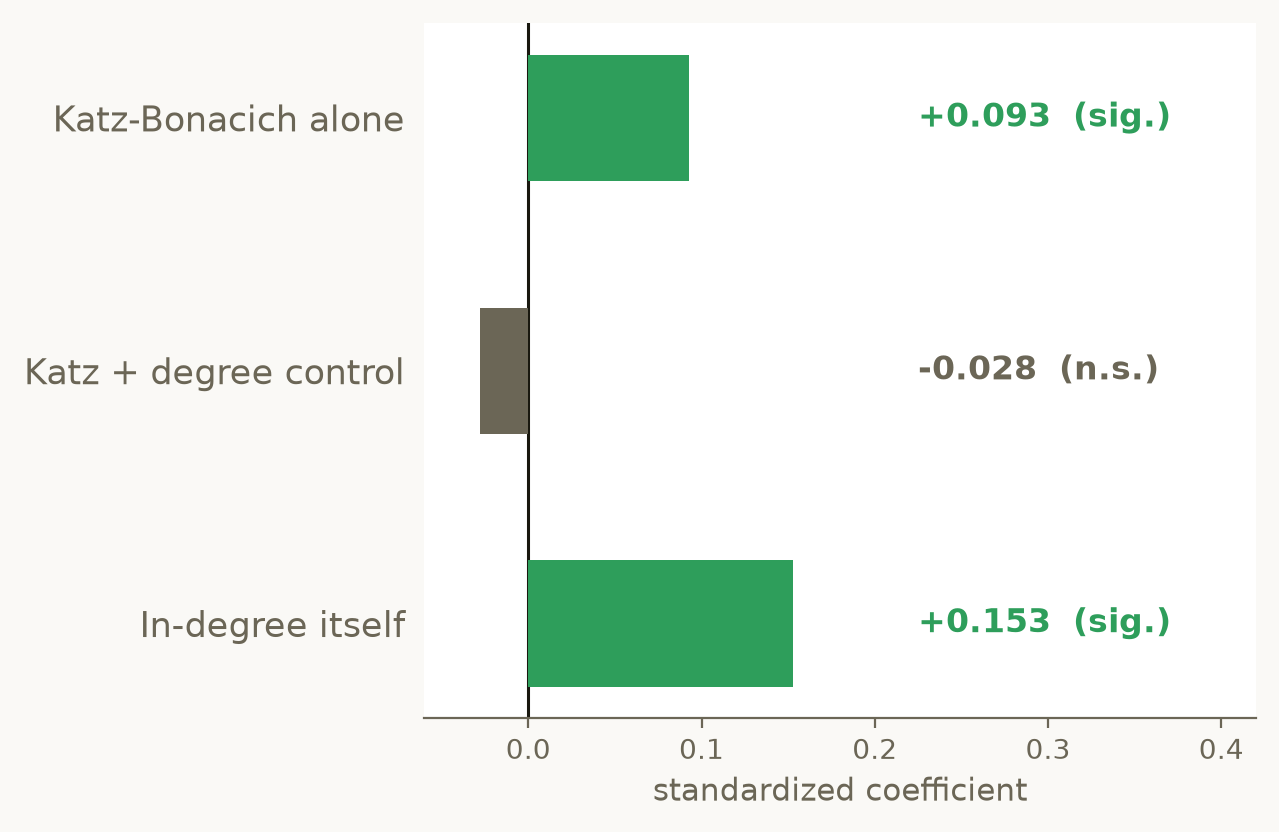
\includegraphics[height=0.6\textheight]{figures/fig_p2_naive_reveal.png}
  \Takeaway{In-degree itself: \(+0.153\), \(p<0.001\) --- that's what was
    driving the naive result.}
\end{frame}

% ---- 6. Result 3a: headline at face value ----
\begin{frame}{The headline test}
  \framesubtitle{Net of popularity and friend GPA, pooled across all 5 groups}
  \medskip
  \centering
  \begin{tabular}{lrrrrrr}
    \toprule
    \(\phi\) (frac.\ of ceiling) & 0.05 & 0.20 & 0.40 & 0.60 & 0.80 & 0.95\\
    \midrule
    Katz coefficient & $+0.082$ & $+0.022$ & $-0.034$ & $-0.051$ & $-0.048$ & $-0.036$\\
    \(p\)-value & $0.012$ & $0.598$ & $0.407$ & $0.115$ & $0.031$ & $0.011$\\
    \bottomrule
  \end{tabular}
  % Source: progress_brief.tex, Result 3 (sweep table + headline paragraph)
  \Takeaway{At \(\phi=0.85\), fixed in advance as the headline: \ResultThreeSlide.
    Read at face value: position has a small, negative, independent effect.}
\end{frame}

% ---- 7. Result 3b: the gap ----
\begin{frame}{But we found a gap in it}
  \framesubtitle{Own-past-GPA cannot be built as a regressor, pooled}
  \centering
  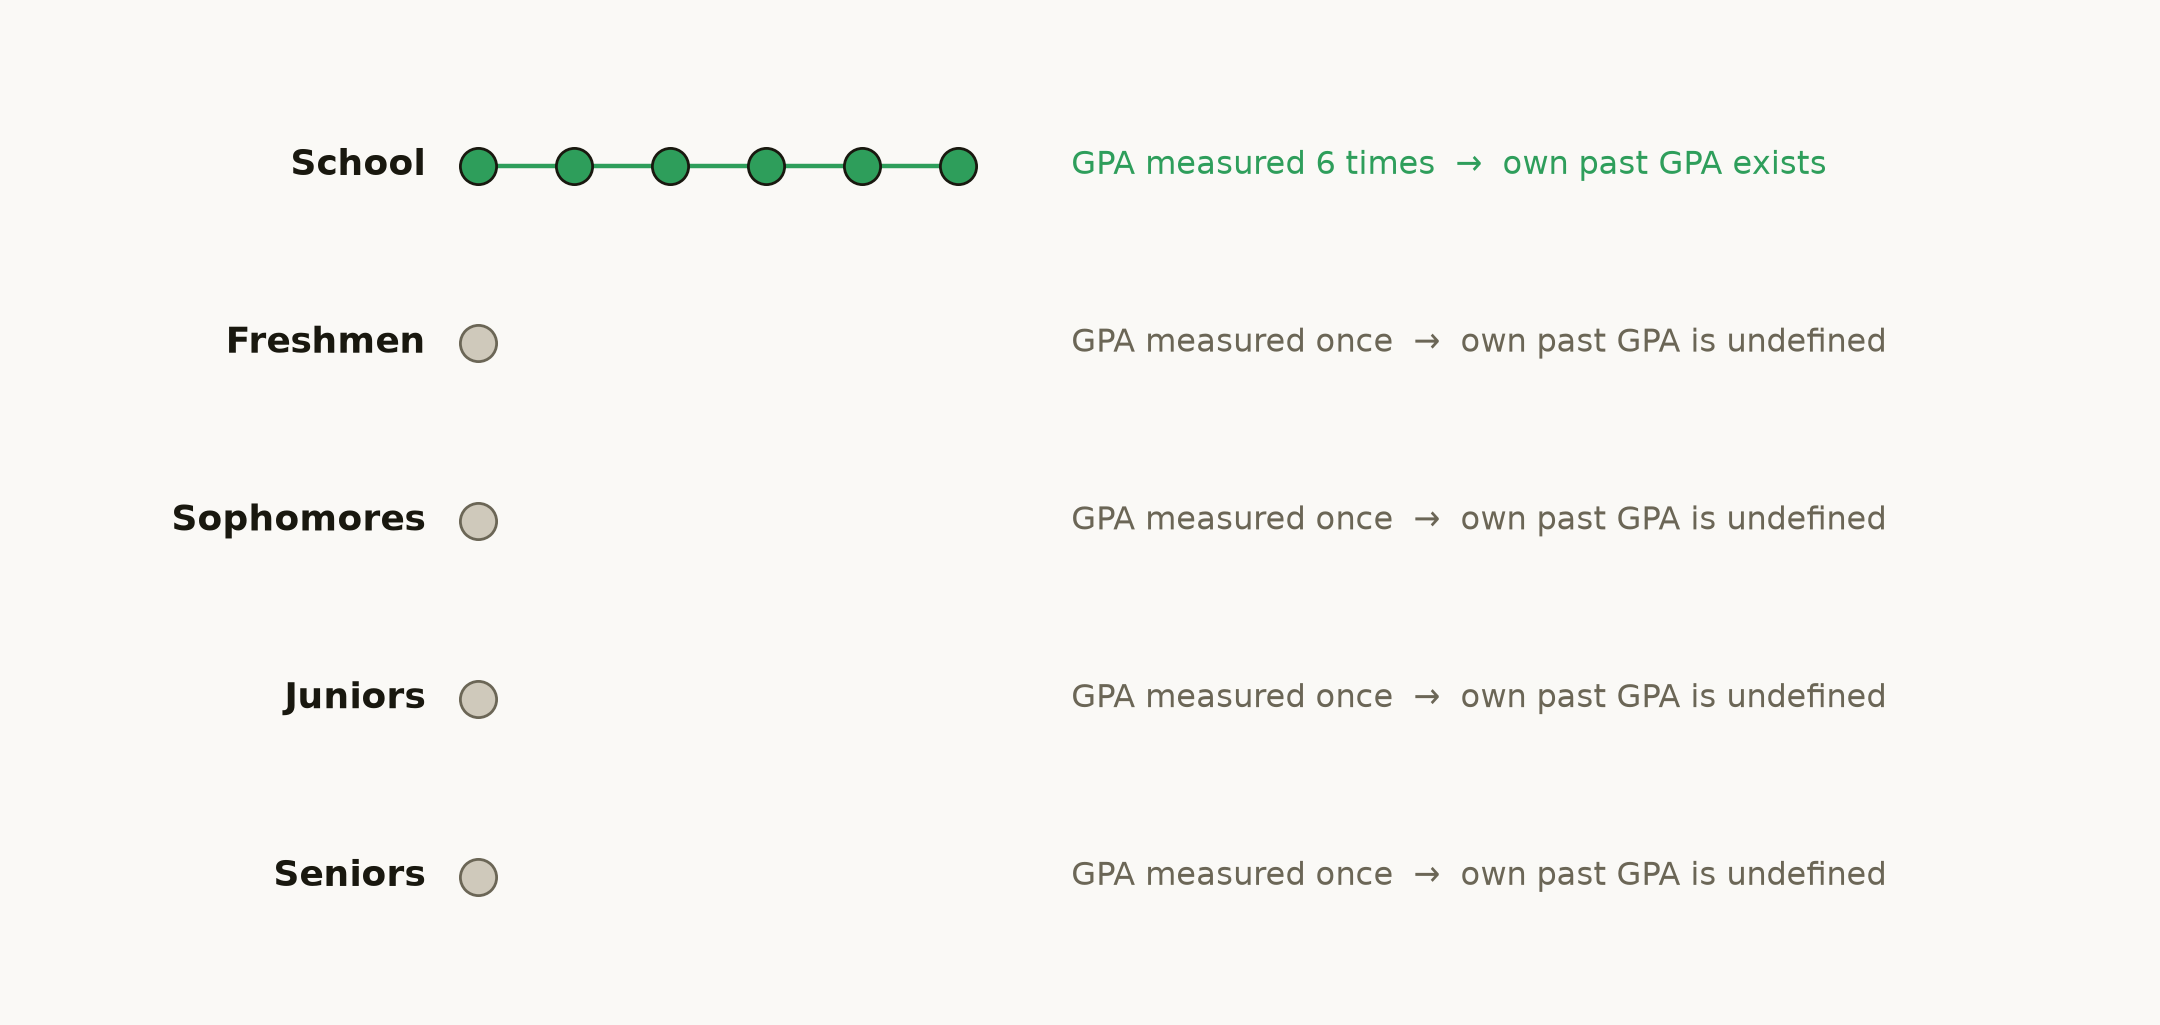
\includegraphics[height=0.58\textheight]{figures/fig_p2_gpa_gap.png}
  \Takeaway{Presentation 1's model equation promised this control. The test
    we actually ran did not have it.}
\end{frame}

% ---- 8. Result 4: the corrected test (load-bearing) ----
\begin{frame}{The corrected test}
  \framesubtitle{School only --- the one sample where a genuine \(t\to t{+}1\)
    design with an own-GPA control is possible}
  \hypertarget{main:result4}{}%
  \centering
  
\includegraphics[height=0.53\textheight]{figures/fig_p2_three_specs.png}
  \TakeawayWithNav{\ResultHeadlineSlide{} (\(n=2{,}088\), 535 students --- a
    much wider confidence interval than the pooled 36,696, but the only
    sample where the test is valid).}
  \PlaceNav{\hyperlink{app:robust}{\beamergotobutton{Robustness}}\;%
    \hyperlink{app:vif}{\beamergotobutton{Multicollinearity}}\;%
    \hyperlink{app:next}{\beamergotobutton{What's next}}}
\end{frame}

% ---- 9. Conclusion ----
\begin{frame}{Conclusion}
  \medskip
  \begin{itemize}\setlength{\itemsep}{1.0em}
    \item \KeyIdea{\ResultHeadlineSlide.}
    \item \textbf{Why this is still worth reporting:} \ResultSupportSlide.
  \end{itemize}
  \bigskip
  \textbf{Implication:} \ResultImplicationSlide. Next: testing whether weak,
  one-way ``likes'' are the reason we see no effect.
  % Deliberately no navigation on the final slide; no "Thank you" slide.
\end{frame}

% ================= Appendix =================
\AppendixStart

\begin{frame}[t]{Sample and network construction}
  \hypertarget{app:sample}{}%
  \medskip
  \begin{itemize}\setlength{\itemsep}{0.6em}
    \item \RunIn{Source:} Smirnov \& Thurner (2017) replication data, Harvard
      Dataverse, CC0. \(\sim\)6{,}200 Russian students.
    \item \RunIn{Nodes:} 655 high-school students; 1{,}200--1{,}549 per
      university cohort (freshmen/sophomores/juniors/seniors).
    \item \RunIn{Edges:} directed ``like'' ties, \(i\to j\) if \(i\) liked
      \(j\) at least once in a \(\sim\)3-month window. 2--14 snapshots per
      group, 38 networks total. Only 24--27\% of ties go both ways.
    \item \RunIn{GPA measurement:} 6 repeated measurements for school; 1
      static measurement for each university cohort.
  \end{itemize}
  \BackButton{main:datarecap}
\end{frame}

\begin{frame}{Robustness: the full \(\phi\) range}
  \hypertarget{app:robust}{}%
  \centering
  
\includegraphics[height=0.6\textheight]{figures/fig_p2_phi_compare.png}
  \Takeaway{Before the fix, pooled swings from significantly positive to
    significantly negative. After it, school-only is flat across the whole
    range.}
  \BackButton{main:result4}
\end{frame}

\begin{frame}[t]{Checking for multicollinearity}
  \hypertarget{app:vif}{}%
  \framesubtitle{Does adding own-past-GPA collide with the other regressors?}
  \medskip
  Own-past-GPA correlates weakly with the other right-hand-side variables:
  \begin{center}
  \begin{tabular}{lrrrr}
    \toprule
    Correlates with & Katz & In-degree & Out-degree & Friend GPA\\
    \midrule
    Correlation & $0.008$ & $0.065$ & $0.122$ & $0.285$\\
    \bottomrule
  \end{tabular}
  \end{center}
  \medskip
  Variance inflation factor for own-past-GPA: \textbf{1.11} --- no
  collinearity problem.
  \Takeaway{Katz and in-degree still correlate at $0.866$ (VIF \(\approx4\))
    --- expected, and exactly what sweeping \(\phi\) is for.}
  \BackButton{main:result4}
\end{frame}

\begin{frame}{What's next: reciprocal ties}
  \hypertarget{app:next}{}%
  \centering
  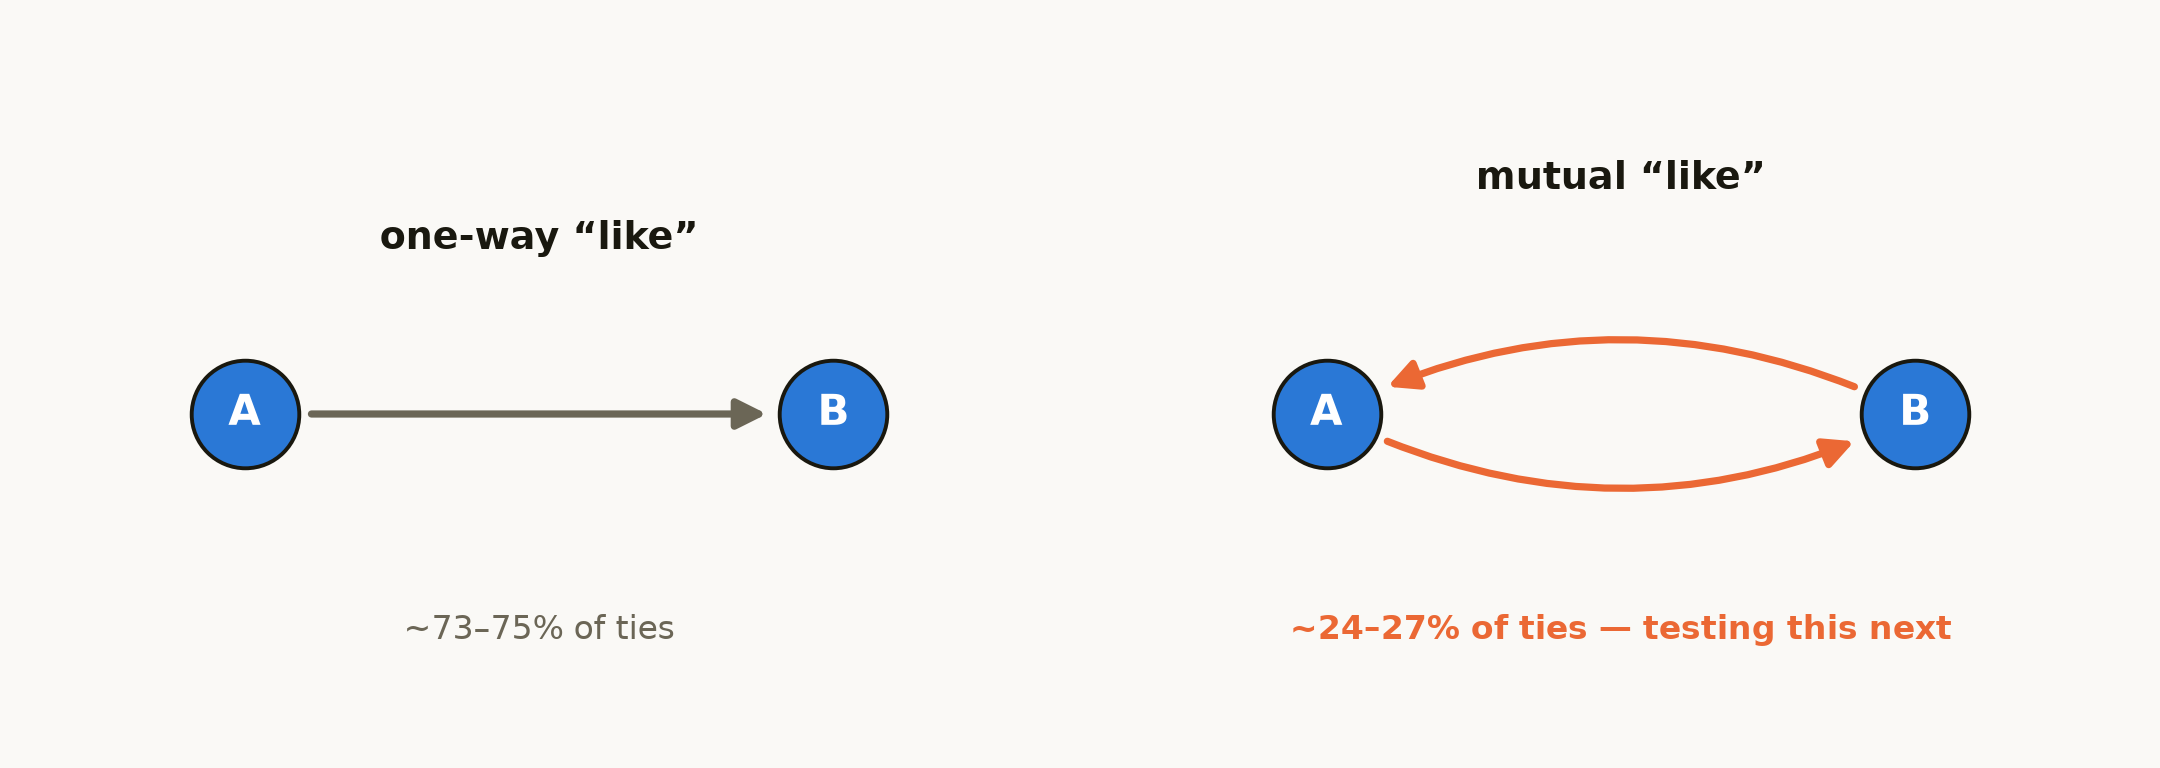
\includegraphics[height=0.55\textheight]{figures/fig_p2_reciprocal_ties.png}
  \Takeaway{Recompute centrality using only mutually-confirmed ties ---
    testing directly whether weak, one-way ``likes'' are the reason we see
    no effect.}
  \BackButton{main:result4}
\end{frame}

\begin{frame}[t]{Related literature}
  \hypertarget{app:lit}{}%
  \medskip
  \begin{itemize}\setlength{\itemsep}{0.65em}
    \item \RunIn{Calv\'o-Armengol, Patacchini \& Zenou (2009), IZA DP 3859:}
      the model we test, on US AddHealth data, one snapshot --- cause and
      effect not separated.
    \item \RunIn{Smirnov \& Thurner (2017), PLOS ONE:} the paper and data we
      replicate and extend; their method looks at one number, a friend's
      average GPA.
    \item \RunIn{Giulietti, Vlassopoulos \& Zenou (2020), IZA DP 13680:} peer
      effects via reference groups, not friendship ties.
  \end{itemize}
  \bigskip
  \textbf{Positioning:} this is the first time Katz--Bonacich centrality has
  been tested with a real time lag and an own-performance control ---
  Calv\'o-Armengol et al.'s cross-sectional data could not support that.
  \BackButton{main:keyq}
\end{frame}

\end{document}
